\begin{table*}[t]
\caption{Held-out results without human labels. PD: profile-determined cases, whose correct label under P1 is \emph{Disjoint applicability} because an instruction file is off the target's chain (B2 computes this in code). Other columns need no reference. Cost: mean calls / mean output tokens per case.}
\label{tab:results}
\centering\footnotesize
\begin{tabular}{lcccccccc}
\toprule
 & PD correct & False conflicts & Called conflict & Order controls & \multicolumn{2}{c}{Prediction changed in variants} & Cost \\ \cmidrule(lr){6-7}
Method & (orig.+var.) & on PD (all) & (orig.+var.) & same prediction & target path & placement & calls / tokens \\
\midrule
B0 & -- & 2/26 & 2/54 & -- & -- & -- & 0.0 / 0 \\
B1 & 21/21 & 0/26 & 0/54 & 23/27 & 8/16 & 5/11 & 1.0 / 2177 \\
B2 & 21/21 & 0/26 & 0/54 & 23/27 & 7/16 & 1/11 & 1.3 / 3589 \\
B1R & 21/21 & 0/26 & 0/54 & 23/27 & 11/16 & 3/11 & 2.0 / 3960 \\
\bottomrule
\end{tabular}
\end{table*}


\textbf{Reference without human labels.} Human labeling was not carried out for this submission, and no model output
substitutes for it. Accuracy is therefore reported only where P1 alone fixes the label: \NPD{} cases (\NPDOrig{}
originals, \NPDVar{} target-path variants, \NPDCtrl{} order controls) in which one instruction's file is not on the
target's directory chain, so that instruction is not loaded and the label is \emph{Disjoint applicability}. B2 computes
the loaded set in code, so on these cases it is correct by construction unless extraction fails; the open question is
whether B1 and B0 also get them right. All other measures in Table~\ref{tab:results} need no reference. This analysis was
defined and frozen by hash before the sealed predictions were opened.

\textbf{Directory scope (RQ2, determined subset).} B1, B2, and B1R each labeled all \NPDMain{} profile-determined
originals and variants correctly (\PrimaryBTwoOnly{} cases favored B2 and \PrimaryBOneOnly{} favored B1), so the direct
model inferred directory applicability from the paths and the profile text without a deterministic step. B0, which
ignores scope, flagged \BZeroPDFalseConf{} of the \NPD{} cases as conflicts: one ESM/CommonJS keyword match between two
unrelated packages, in the original and in its order control. For this model, the determined subset does not support
the hypothesis that explicit structure is needed to handle directory scope.

\begin{figure}[t]
\centering
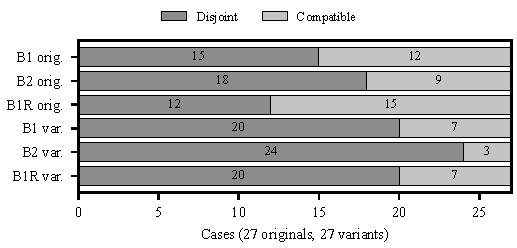
\includegraphics[width=\columnwidth]{build/figures/labels.pdf}
\caption{Predicted labels per model arm on the \NOriginals{} originals and \NVariants{} variants (counts; not accuracy).
No arm predicted \emph{Unresolved conflict}, \emph{Valid override}, or \emph{Insufficient evidence}.}
\label{fig:labels}
\end{figure}

\textbf{Label-free comparison.} No model arm labeled any original or variant an unresolved conflict or a valid
override; every prediction was \emph{Compatible} or \emph{Disjoint} (Fig.~\ref{fig:labels}), while B0 flagged
\BZeroCalledConfAnn{} of the 54. The challenge-oriented retrieval thus surfaced lexically similar pairs that the models
judged non-conflicting. The arms differ on the boundary between compatibility and condition-limited applicability: on
originals B2 chose \emph{Disjoint} \BTwoDistOrigDisjoint{} times and B1 \BOneDistOrigDisjoint{} times; B1 and B2
agreed on \AgreeBOneBTwoOrigSame{} of 27 originals (Cohen's $\kappa = \AgreeBOneBTwoOrigKappa$) and
\AgreeBOneBTwoVarSame{} of 27 variants ($\kappa = \AgreeBOneBTwoVarKappa$). The first non-determined original on which
they disagree (by the declared selection rule) pairs a root rule ``use \texttt{Protocol} for decoupling'' with a nested
rule ``avoid \texttt{TYPE\_CHECKING}'', both Python-specific, for a TypeScript target. B1 treated both rules as
inactive; B2's extraction found no explicit condition and returned \emph{Compatible}. Which reading is right is a
judgment about implicit applicability that P1 does not settle and that human labels must resolve.

\textbf{Stability and sensitivity (RQ3).} Swapping only the order of the two instructions changed the label in four of
\NControls{} controls for each model arm (\BOneOrderStable{}, \BTwoOrderStable{}, and \BOneROrderStable{} unchanged for
B1, B2, and B1R), although all \NPDCtrl{} determined controls stayed correct. All \NVarTarget{} target-path variants,
which move the target out of the nested file's directory, were labeled \emph{Disjoint} by every arm; the label differed
from the original's in \BOneTVChanged{} (B1), \BTwoTVChanged{} (B2), and \BOneRTVChanged{} (B1R) cases, because many
originals were already judged inactive by condition. Placement variants changed B2's label \BTwoPVChanged{} time and
B1's \BOnePVChanged{} times out of \NVarPlacement{}; without reference labels we cannot say which changes are correct.

\textbf{Cost.} No arm had a failure, retry, or malformed output. B2 averaged \BTwoCallsPerCase{} calls and
\BTwoMeanOut{} output tokens per case, against \BOneCallsPerCase{} and \BOneMeanOut{} for B1; the equal-call control B1R
(\BOneRMeanOut{} tokens) changed its first answer in \BOneRReviewChanged{} of 81 cases. Latency is not compared because
the GPU was shared with another process for part of the runs.
